\section{Verteilte Anwendungen mit RMI}

Wenn man eine verteilte Java-Anwendung entwickeln soll, bei der Kommunikationsprotokoll und Client- und Server-Seite in Java implementiert werden, ist \textbf{RMI} die bessere Alternative gegenüber  \textbf{Sockets} (vgl.~\cite[311]{Oec22}).\\


\begin{tcolorbox}
    \textbf{Remote Method Invocation} ermöglicht das Aufrufen von Methoden auf Objekten, die sich auf demselben oder einem anderem Rechner als der Aufrufer befinden, und damit als unterschiedliche Prozesse in unterschiedlichen Adressräumen ausgeführt werden.
\end{tcolorbox}

\noindent
\textbf{Remote Method Invocation} (RMI) stellt eine Schnittstelle zur Nutzung der Internetprotokolle \textbf{TCP} und \textbf{UDP} bereit.\\

\noindent
\textbf{RMI} verfolgt den Ansatz, OOP auch für die Kommunikation zwischen verteilten Anwendungen zu realisieren, wobei der Aspekt der Verteilung für die Entwickler weitestgehend transparent bleibt

\begin{figure}
    \centering
    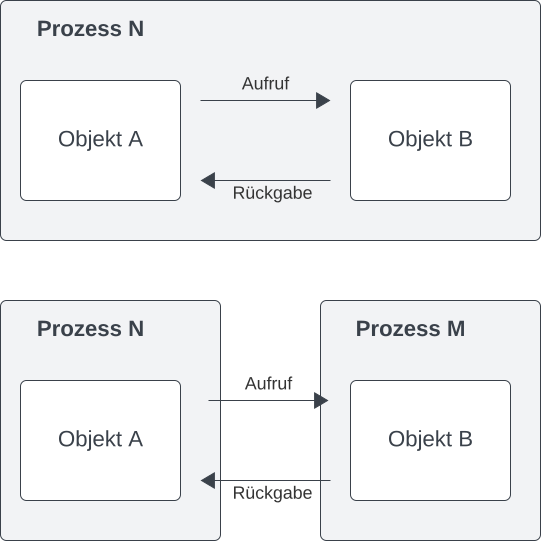
\includegraphics[scale=0.5]{chapters/fopt5/img/rmi/processcall}
    \caption{Zwei unterschiedliche Objekte in unterschidlichen Aufrufsituationen. Im oberen Beispiel befinden sich die Objekte im selben Adressraum, im unteren Beispiel in unterschiedlichen Adressräumen - diese Situation kommt bei der Nutzung von RMI vor (Quelle: in Anlehnung an \cite[311 f., Abbildung 6.1 und 6.2]{Oec22})}
    \label{fig:processcall}
\end{figure}

\noindent
Die \textbf{Vereilungstransparenz} wird bei \textbf{RMI} über \textbf{Stubs} und \textbf{Skeletons} realisiert.\\

\noindent
Ein \textbf{Stub} implementiert dieselbe Schnittstelle wie das Objekt, das über Fern-Methodenaufrufe \ul{auf dem Server gesteuert werden soll}.

\noindent
Ein \textbf{Skeleton} nimmt die Nachrichten, die vom \textbf{Stub} über die aufgebaute \textbf{TCP}-Verbindung gesendet werden, entgegen und ruft die Methoden auf dem entsprechenden Server-Objekt auf.\\
$\rightarrow$ Ein \textbf{Skeleton} besitzt die Struktur eines \textbf{TCP}-Servers.

\begin{figure}
    \centering
    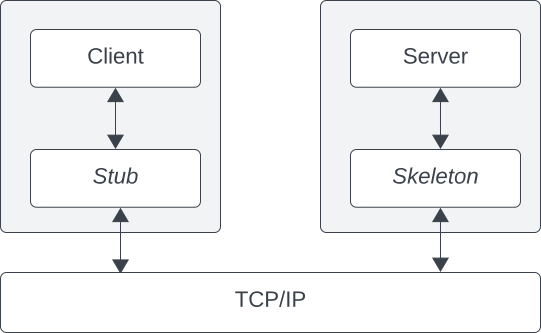
\includegraphics[scale=0.4]{chapters/fopt5/img/rmi/stubskeleton}
    \caption{Prinzip der Kommunikation zwischen RMI-Client und -Server. (Quelle: in Anlehnung an \cite[312, Bild 6.3]{Oec22})}
    \label{fig:stubskeleton}
\end{figure}

\begin{tcolorbox}
    Struktur einer RMI Anwendung\footnote{vgl. im folgenden \cite[162 ff.]{HM05}; \textbf{Stubs} und \textbf{Skeletons} werden automatisch generiert.}:\\


    \noindent
    \textbf{RMI-Client}\\
    Ein \textbf{RMI-Client} fragt bei einem \textbf{RMI-Namensdienst} eine Referenz auf ein entferntes Objekt an, das danach wie ein lokales Objekt behandelt wird.
    Die notwendige Netzwerk-Kommunikation für diese Methodenaufrufe ist transparent und wird automatische abgewickelt.\\


    \noindent
    \textbf{Stub-Objekt}
    \begin{itemize}
        \item Ein \textbf{Stub-Objekt} ist ein \textbf{Stellvertreter} für das entfernte Objekt bei dem RMI-Server.
        Methodenaufrufe des \textbf{RMI-Clients} auf ein entferntes Objekt werden an das Stub-Objekt \textit{delegiert}.
        \item Verantwortlichkeiten: Weiterleitung von Methodenaufrufe an das entfernte Objekt. \textit{Marshalling} von Übergabeparametern und \textit{unmarshalling} von Rückgabewerten\footnote{
          Serialisierung: Umwandeln einer Objektstruktur in ein speicherbares Format. Marshalling bezieht sich auf das Bewegen von Objekten zwischen Threads und Programmen, wofür auch eine Form von Serialisierung notwendig ist. S. a. ``Marshalling (computer science): \url{https://en.wikipedia.org/wiki/Marshalling_(computer_science)} - abgerufen 1.2.2024
        }.
        \item Der Stub wird für jede Anwendung automatisch erzeugt (vgl.\cite[313]{Oec22}).
    \end{itemize}\\

    \noindent
    \textbf{Skeleton-Objekt}\\
   Ein \textbf{Skeleton-Objekt} ist ein \textit{server-seitiger} \textbf{Stellvertreter} für das aufrufende Objekt bei dem RMI-Server, uns unterstützt ebenfalls  \textit{Marshalling} von Übergabeparametern und \textit{unmarshalling} von Rückgabewerten. Das Sekeleton-Objekt ist als Programmteil in der RMI-Implementierung dabei und kann für alle RMI-Anwendungen verwendet werden (vgl.\cite[313]{Oec22}).\\

    \noindent
    \textbf{RMI-Registry}\\
    Die \textbf{RMI-Registry} realisiert einen \textit{Namensdienst}: Eine Abbildung von Namen auf entfernte Objekte.\footnote{
        s.a: ``Kapitel 6: Verteilte Objekte durch RMI``: \url{https://www.informatik.uni-marburg.de/~mathes/download/k6.pdf}, ``Distributed object communication``: \url{https://en.wikipedia.org/wiki/Distributed_object_communication} - beides abgerufen 1.2.2024
    }. \\
    Der \textbf{RMI-Client} fordert hier die Referenzen auf entfernte Objekte an.\\

    \noindent
    \textbf{RMI-Server}\\
    Ein \textbf{RMI-Server} instanziiert ein entferntes Objekt und registriert es unter einem Namen bei der \textbf{RMI-Registry}, und wartet \textit{passiv} auf den Aufruf einer Methode durch den \textbf{RMI-Client}.

\end{tcolorbox}

\begin{figure}
    \centering
    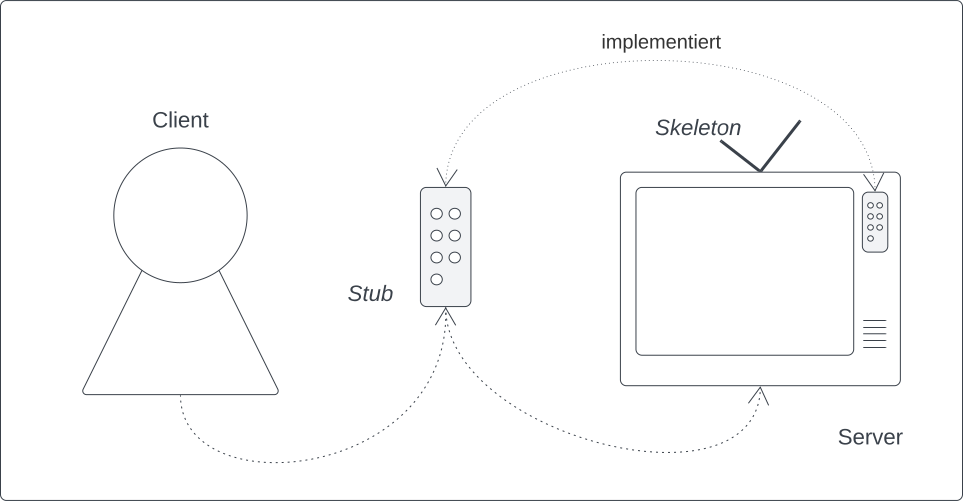
\includegraphics[scale=0.35]{chapters/fopt5/img/rmi/tv}
    \caption{Eine Illustration der im Lehrbuch verwendeten RMI-Metapher. Ein Client will ein entferntes Objekt (TV) bedienen. Hierzu verwendet er Methodenaufrufe, die vom Stub (Fernbedienung) weitergeleitet werden. Die Methoden werden vom Skeleton (Fensehantennen) an das Objekt auf dem Server weitergeleitet. Dieses Objekt sind in dem Beispiel die Knöpfe an dem Fernseher, die die gleichen Bedienfunktionen (``Schnittstelle``) wie die Fernbedienung haben. (Quelle: eigene)}
    \label{fig:tv}
\end{figure}

\noindent
Die \textbf{Transparenz} kommt für den Entwickler dadurch zustande, dass er nur Client und Server, nicht aber Stub und Skeleton programmieren muss.\\
$\rightarrow$ \textbf{Stub} wird automatisch erzeugt, das \texbf{Skeleton}-Objekt ist ein Programmteil, der in der \textbf{RMI}-Implementierung dabei ist und für alle Anwendungen verwendet werden kann.\\

\noindent
Die Entwicklung einer \textbf{RMI}-Anwendung erfolgt i.d.R. in folgenden Schritten\footnote{
s.a. ``An Overview of RMI Applications``: \url{https://docs.oracle.com/javase/tutorial/rmi/overview.html} - abgerufen 1.2.2024
}:

\begin{enumerate}
    \item\label{itm:intdef} \textbf{Schnittstelle definieren}\\
    \noindent
    Die Schnittstelle zwischen Client & Server in Abhängigkeit von der Anwendung, die realisiert werden soll.\\
    \noindent
    Die Schnittstelle führt alle Methoden auf, die über \textbf{RMI} aufgerufen werden sollen.\\
    \noindent
    Die Schnittstelle muss aus \code{java.rmi.Remote} abgeleitet werden.\\
    \noindent
    Alle Methoden der Schnittstelle müssen mit \code{throws RemoteException} gekennzeichnet werden\footnote{
    s.a. ``2.4.1 The java.rmi.Remote Interface``: \url{https://docs.oracle.com/en/java/javase/21/docs/specs/rmi/objmodel.html#the-java.rmi.remote-interface} - abgerufen 1.2.2024
    }.

    \item \textbf{Schnittstelle implementieren}\\
    \noindent
    Es wird eine Klasse geschrieben, die die im ersten Schritt definierte Schnittstelle implementiert.\\
    \noindent
    Einem Objekt davon muss \ul{von aussen über RMI} nutzbar sein - es muss exportiert werden können.
    Dazu kann die implementierende Klasse von \code{UnicastRemoteObject} abgeleitet werden.\\
    Es muss ein expliziter Konstruktor existieren, der mit \code{throws RemoteException} gekennzeichnet wird. \\
    $\rightarrow$ Es muss mindestens ein expliziter Standard-Konstruktor existieren, der diese Bedingung erfüllt\footnote{
    ansonsten wird vom Compiler ein Standard-Konstruktor zur Verfügung gestellt.
    Da dieser aber keine checked Exception in Form einer \textit{RemoteException} wirft, kommt es zu einem Compilerfehler.
    }

    \item \textbf{Server programmieren}\\
    \noindent
    Man erzeugt eines oder mehrere Objekte der in Schritt 2 implementierten Klasse und meldet diese unter einem beliebigen Namen bei der \textbf{RMI-Registry} an.

    \item \textbf{Client programmieren}\\
    \noindent
    Über die \textbf{RMI-Registry} (Serveradresse und Port müssen dem Client bekannt sein) beschafft sich der Client die in Schritt 3 registrieren Objekte, die als \textbf{Stub} an ihn weitergeleitet werden.\\
    \noindent
    Der Stub kann unter Berücksichtigung der in Schritt 1 definierten Schnittstelle so verwendet werden, als wäre es ein lokales Objekt\footnote{
    ``lokal`` im Sinne von gleicher Prozess / gleicher Adressraum.
    }.\\
    \noindent
    Die Methodenaufrufe werden dann letztendlich auf dem durch das in Schritt 2 definierte \textbf{RMI-Objekt} auf dem Server ausgeführt (Client $\rightarrow$ Stub $\rightarrow$ Skeleton $\rightarrow$ Server).

    \item \textbf{Anwendung übersetzen und ausführen}\\
    \noindent
    Alle Dateien werden kompiliert.
    Vor dem Starten des Programms ist darauf zu achten, dass auf dem Server die \textbf{RMI-Registry} gestartet wird - was aber auch aus dem Programm heraus geschehen kann.
\end{enumerate}

\section{Einführendes RMI-Beispiel}

Auch bei RMI-Implementierungen bei denen mehrere Clients gleichzeitig auf eine Objektinstanz zugreifen, ist (ggfl. nach Anwendung) \code{synchronized} nötig, um ein Objekt für den gleichzeitigen Zugriff zu sperren.\\

\noindent
Sobald über \staticcode{java.rmi.Naming.rebind()} bzw. \staticcode{bind()}\footnote{
textit{bind()} wirft eine \textit{AlreadyBoundException}, falls in der RMI-Registry bereits ein Eintrag mit dem Namen existiert, \textit{rebind()} hingegen ersetzt einen ggf. breits existierenden Eintrag mit gleichem Namen.
} der Server gestartet wurde, wird ein Thread gestartet, der den Skeleton repräsentiert, auf eingehende TCP-Verbindungen wartet.\\

\noindent
der Client frag vom Server über

\begin{minted}[mathescape,
    linenos,
    numbersep=5pt,
    gobble=2,
    frame=lines,
    framesep=2mm]{java}
    java.rmi.Naming.lookup("rmi://serveradresse/bindingname");
\end{minted}\\

das Objekt ab, auf das er zugreifen möchte, und bekommt dann ein Objekt vom Typ \code{java.rmi.Remote} zurück.\\
Das Objekt muss noch zu dem Typen gecasted werden, der in ``Schnittstelle definieren`` in Punkt~\ref{itm:intdef} (s. vorheriger Abschnitt) implementiert wurde, um entsprechende Methoden der implementierten Schnittstelle aufrufen zu können - \ul{das über }\code{lookup()}\ul{ zurückgegebene Objekt ist das \textbf{Stub-Objekt}}.\\

\noindent
Bevor der Server auf dem entsprechenden Rechner gestartet wird, muss auf diesem Rechner über die Konsole noch \code{rmiregistry} aufgerufen werden, damit die \textbf{Registry} zur Verfügung steht, sofern das nicht wie im folgenden Beispiel über das Programm geschieht.\\

Im Folgenden ein Beispiel für ein komplettes RMI-Programm, das einen einfachen Echo-Server\footnote{
``Echo Protocol``: \url{https://en.wikipedia.org/wiki/Echo_Protocol} - abgerufen 2.2.2024
} implementiert.
Die RMI-Registry wird hierbei ebenfalls über das Programm gestartet.
\begin{minted}[mathescape,
linenos,
numbersep=5pt,
gobble=2,
fontsize=\small,
frame=lines,
framesep=2mm]{java}
    public class RMIDemo {

        interface Echo extends Remote {
            String echo(String msg) throws RemoteException;
        }

        static class EchoImpl extends UnicastRemoteObject implements Echo {

            public EchoImpl() throws RemoteException{}

            @Override
            public String echo(String msg) throws RemoteException {
                return msg;
            }
        }

        public static void main(String[] args) {

            if (args.length == 0) {
                // Server
                try {
                    Registry registry = LocateRegistry.createRegistry(1099);
                    registry.rebind("echo", new EchoImpl());
                } catch (RemoteException e) {
                    System.err.println("[registry] " + e);
                }
                //Thread is started, it's okay to leave main() at this point.
                return;
            }

            // client
            try {
                Remote stub = Naming.lookup("rmi://localhost:1099/echo");
                Echo echo = (Echo) stub;
                System.out.println(echo.echo(args[0]));
            } catch (NotBoundException | MalformedURLException | RemoteException e) {
                System.err.println("[client] " + e);
            }
        }
    }
\end{minted}\\

\begin{tcolorbox}
    RMI-Methodenaufrufe sind blocking, auch wenn der Rückgabetyp für die aufgerufene Methoden mit \code{void}-deklariert wurde.\\

    \blockquote[{``3.1 Stubs and Skeletons``: \url{https://docs.oracle.com/en/java/javase/21/docs/specs/rmi/arch.html} - abgerufen 2.2.2024 (Hervorherbungen eigene)}]{
        When a stub's method is invoked, it does the following:
        \begin{itemize}
            \item initiates a connection with the remote JVM containing the remote object,
            \item marshals (writes and transmits) the parameters to the remote JVM,
            \item \textbf{waits for the result of the method invocation},
            \item \textbf{unmarshals (reads) the return value or exception returned}, and
            \item returns the value to the caller.
        \end{itemize}

    }
\end{tcolorbox}

\subsection{RMI-Client mit grafischer Benutzeroberfläche}

In dem Beispiel \cite[320, Listing 6.5]{Oec22} wird bei jedem Buttonclick ein neuer Thread gestartet.
Die gestarteten Threads können unterschiedlich schnell ablaufen, und somit zu unerwarteten Ergebnissen führen:

\blockquote[{\cite[323]{Oec22}}]{
[...], aber man wird vermutlich davon ausgehen, dasss der angezeigte Zählerwert immer derjenige ist, der aus der eigenen zuletzt angestoßenen Aktion resultiert.
    Aber dies muss nicht in jedem Fall so sein.
}

Als Lösung könnte man die ankommenden Aufträge durch einen einzigen Thread ausführen lassen, indem die Aktionen {bspw.} in eine Warteschlange eingereiht werden (vgl.~\cite[323]{Oec22}).

\newpage
In dem o.a. Listing wird das Functional Interface \Code{Consumer}\footnote{
`´Interface Consumer<T>``: \url{https://docs.oracle.com/en/java/javase/21/docs/api/java.base/java/util/function/Consumer.html} - abgerufen 2.2.2024
} verwendet.
Folgendes Beispiel stellt die Verwendung in vereinfachter Form nochmal dar:


\begin{minted}[mathescape,
    linenos,
    numbersep=5pt,
    gobble=2,
    fontsize=\small,
    frame=lines,
    framesep=2mm]{java}
    public class ConsumerDemo {
        interface Supplier<T> {
            T execute();
        }

        public <T> void asyncCall(Supplier<T> s, Consumer<T> c) {
            startThread(s, c);
        }

        public <T> void startThread(Supplier<T> s, Consumer<T> c) {
            Thread t = new Thread(() -> c.accept(s.execute()));
            t.start();
        }

        public static void main(String[] args) {
            ConsumerDemo cd = new ConsumerDemo();
            cd.asyncCall(
                () -> Math.random() * 100,
                (r) -> System.out.println("Done: " + r)
            );
        }
    }
\end{minted}\\